\documentclass[11pt,a4paper]{article}

% ==================== PACOTES ====================
\usepackage[utf8]{inputenc}
\usepackage[T1]{fontenc}
\usepackage[brazilian]{babel}
\usepackage{geometry}
\geometry{top=2.0cm, bottom=2.2cm, left=2.0cm, right=2.0cm}
\usepackage{graphicx}
\usepackage{float}
\usepackage{hyperref}
\usepackage{enumitem}
\usepackage{booktabs}
\usepackage{array}
\usepackage{amssymb}
\usepackage{xcolor}
\usepackage{listings}
\usepackage{tcolorbox}
\tcbuselibrary{skins,breakable}

% ==================== CORES E ESTILOS ====================
\definecolor{imeblue}{RGB}{0, 51, 102}
\definecolor{alertred}{RGB}{180, 20, 20}
\definecolor{homegreen}{RGB}{20, 110, 50}
\definecolor{theorypurple}{RGB}{90, 40, 130}
\definecolor{armorange}{RGB}{190, 80, 10}
\definecolor{bizucyan}{RGB}{0, 110, 130}
\definecolor{codebg}{RGB}{245, 247, 250}

\hypersetup{
    colorlinks=true,
    linkcolor=imeblue,
    urlcolor=imeblue
}

\lstset{
    backgroundcolor=\color{codebg},
    basicstyle=\ttfamily\small,
    breaklines=true,
    frame=single,
    rulecolor=\color{gray!40},
    showstringspaces=false,
    commentstyle=\color{homegreen},
    keywordstyle=\color{imeblue}\bfseries,
    literate={á}{{\'a}}1 {à}{{\`a}}1 {ã}{{\~a}}1 {â}{{\^a}}1
             {é}{{\'e}}1 {ê}{{\^e}}1 {í}{{\'i}}1 {ó}{{\'o}}1
             {õ}{{\~o}}1 {ô}{{\^o}}1 {ú}{{\'u}}1 {ç}{{\c{c}}}1
             {Á}{{\'A}}1 {É}{{\'E}}1 {Í}{{\'I}}1 {Ó}{{\'O}}1
             {Ú}{{\'U}}1 {Ç}{{\c{C}}}1
}

% Caixas didaticas personalizadas
\newtcolorbox{alertbox}[1]{
    colback=alertred!5!white,
    colframe=alertred,
    fonttitle=\bfseries,
    title={#1},
    breakable
}

\newtcolorbox{theorybox}[1]{
    colback=theorypurple!5!white,
    colframe=theorypurple,
    fonttitle=\bfseries,
    title={#1},
    breakable
}

\newtcolorbox{homebox}[1]{
    colback=homegreen!5!white,
    colframe=homegreen,
    fonttitle=\bfseries,
    title={#1},
    breakable
}

\newtcolorbox{labbox}[1]{
    colback=imeblue!5!white,
    colframe=imeblue,
    fonttitle=\bfseries,
    title={#1},
    breakable
}

\newtcolorbox{armbox}[1]{
    colback=armorange!5!white,
    colframe=armorange,
    fonttitle=\bfseries,
    title={#1},
    breakable
}

\newtcolorbox{bizubox}[1]{
    colback=bizucyan!5!white,
    colframe=bizucyan,
    fonttitle=\bfseries,
    title={#1},
    breakable
}

% ==================== INÍCIO DO DOCUMENTO ====================
\begin{document}

\begin{center}
    {\Large \textbf{INSTITUTO MILITAR DE ENGENHARIA (IME)}}\\[0.15cm]
    {\large Seção de Engenharia Elétrica --- SE/3}\\[0.1cm]
    {\normalsize Programação Aplicada à Engenharia Elétrica (SE/3 - Eletrônica)}\\[0.25cm]
    {\Large \textbf{Manual Mestre de Execução e Aprendizado: Do Zero ao Deploy}}\\[0.1cm]
    {\normalsize \textit{Montagem Física, Ambiente Virtual, Pastas Compartilhadas, WinSCP, POO C++, IIO e Cross-Compilação}}\\[0.35cm]
    \begin{tabular}{lp{11.0cm}}
        \toprule
        \textbf{Instituição:} & Instituto Militar de Engenharia (IME) / SE/3 \\
        \textbf{Missão do Projeto:} & Monitoramento Inteligente de Carga Sensível em Operações Logísticas \\
        \textbf{Kit de Hardware:} & STMicroelectronics \textbf{STM32MP157D-DK1} (Linux Embarcado OpenSTLinux) \\
        \textbf{Sensor Alocado (Nº 3):} & Módulo de Obstáculo Infravermelho Reflexivo Digital (\textbf{HW-201} / LM393) \\
        \textbf{Critério de Avaliação:} & Projeto = 4.000 pontos (VF) em 5 entregas de 800 pts $|$ Listas = 6.000 pontos \\
        \textbf{Prazo Entrega 1:} & \textbf{26/10/2026 às 23:59} --- Classe C++ com Doxygen no Git (800 pontos) \\
        \textbf{Prazo Entrega 2:} & \textbf{02/11/2026 às 23:59} --- Binário ARM Funcional no Kit + README (800 pontos) \\
        \bottomrule
    \end{tabular}
\end{center}

\vspace{0.2cm}

% ====================================================================
\section{Apresentação Geral e Novo Critério Oficial de Notas}
% ====================================================================

Em comunicado recente divulgado no Google Classroom da disciplina (Figura~\ref{fig:notas_sistema}), foram estabelecidas as regras definitivas para o cálculo das notas da disciplina:
\begin{itemize}[leftmargin=*]
    \item \textbf{Escala Global:} Cada aluno pode somar até \textbf{10.000 pontos} na matéria (para evitar dízimas e facilitar pontuações decimais).
    \item \textbf{O Trabalho (Projeto Final):} Vale \textbf{4.000 pontos} divididos em 5 entregas parciais de \textbf{800 pontos} cada. O projeto possui o peso equivalente à \textbf{Verificação Final (VF)}.
    \item \textbf{As Listas de Exercícios:} Somam um total de \textbf{6.000 pontos} distribuídos entre si, equivalendo à \textbf{Verificação Corrente (VC) e Verificações Especiais (VEs)}.
\end{itemize}

\begin{figure}[H]
    \centering
    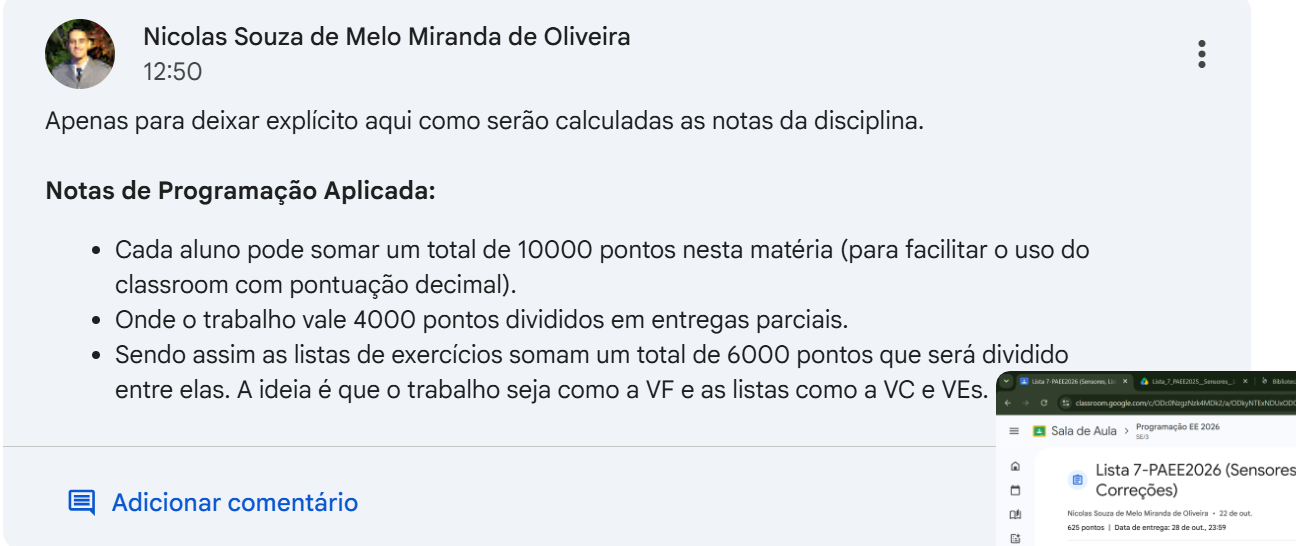
\includegraphics[width=0.88\textwidth]{latex_assets/classroom_notas_sistema.png}
    \caption{Comunicado oficial no Google Classroom detalhando o sistema de pontuação (10.000 pts total; 4.000 pts Projeto; 6.000 pts Listas).}
    \label{fig:notas_sistema}
\end{figure}

\begin{center}
\begin{tabular}{llcp{7.0cm}}
    \toprule
    \textbf{Etapa} & \textbf{Prazo Final} & \textbf{Pontuação} & \textbf{Entregável Principal} \\
    \midrule
    \textbf{Entrega 0} & 19/10/2026 & Concluída & Validação física da montagem com o kit desligado. \\
    \textbf{Entrega 1} & \textbf{26/10/2026} & \textbf{800 pts} & Classe C++ (\texttt{IrObstacleSensor}) com Doxygen no Git. \textbf{Deve rodar na placa!} \\
    \textbf{Entrega 2} & \textbf{02/11/2026} & \textbf{800 pts} & Binário ARM funcional na STM32MP1 + Instruções no README.md. \\
    \textbf{Entrega 3} & 09/11/2026 & \textbf{800 pts} & Telemetria UDP contínua (porta 5000) e protocolo documentado. \\
    \textbf{Entrega 4} & 16/11/2026 & \textbf{800 pts} & Interface gráfica (GUI) no computador com gráfico e exportação CSV. \\
    \textbf{Entrega 5} & 16/11/2026 & \textbf{800 pts} & \textbf{Mesma data da E4!} Vídeo de demonstração e apresentação final. \\
    \bottomrule
\end{tabular}
\end{center}

\begin{alertbox}{Critério Eliminatório de Avaliação: Regra de POO Estrita}
O edital oficial determina: \textbf{é expressamente proibida a utilização de variáveis globais e de funções soltas fora de classes}.
\begin{itemize}[leftmargin=*]
    \item \textbf{A razão de engenharia:} Na fase final, os 11 grupos da turma integrarão seus módulos no servidor central. Variáveis globais ou funções livres causariam conflito de nomes no linker (\textit{symbol collision}).
    \item \textbf{Padrão exigido:} Todos os estados do sensor (caminho de arquivo, último valor, limiares) devem ser atributos \texttt{private}, manipulados unicamente por métodos \texttt{public} bem documentados.
\end{itemize}
\end{alertbox}

\newpage
% ====================================================================
\section{O Hardware: Placa STM32MP157D-DK1 e Sensor HW-201}
% ====================================================================

Antes de manusear os componentes, é indispensável conhecer as características elétricas e arquiteturais dos equipamentos fornecidos:

\begin{figure}[H]
    \centering
    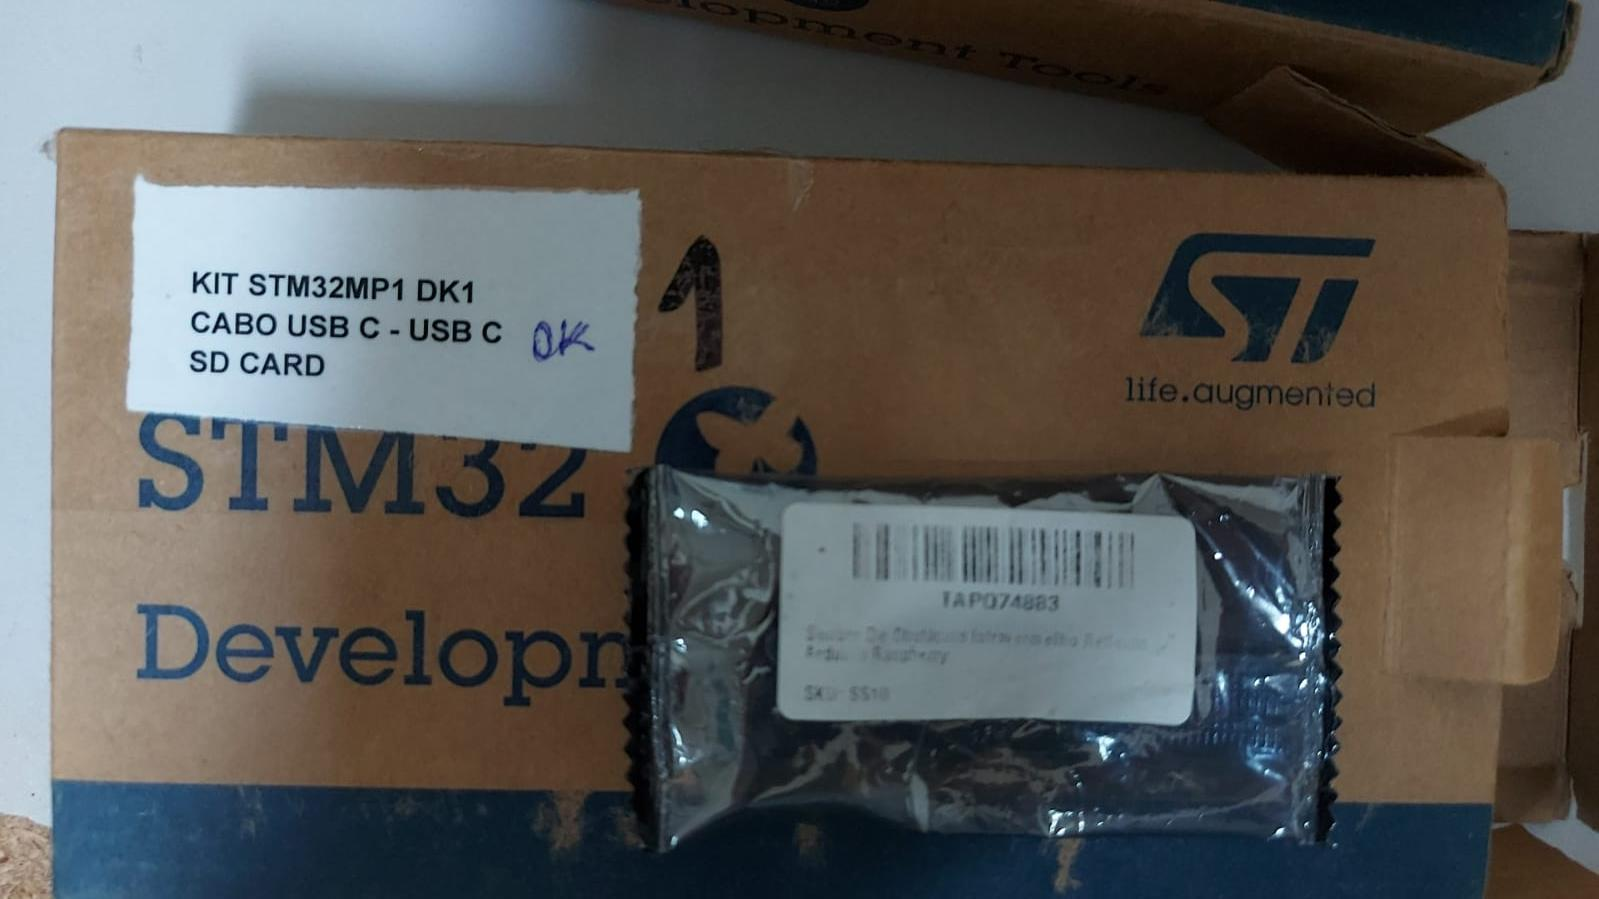
\includegraphics[height=4.6cm]{latex_assets/foto_kit_caixa.jpg}
    \hspace{0.4cm}
    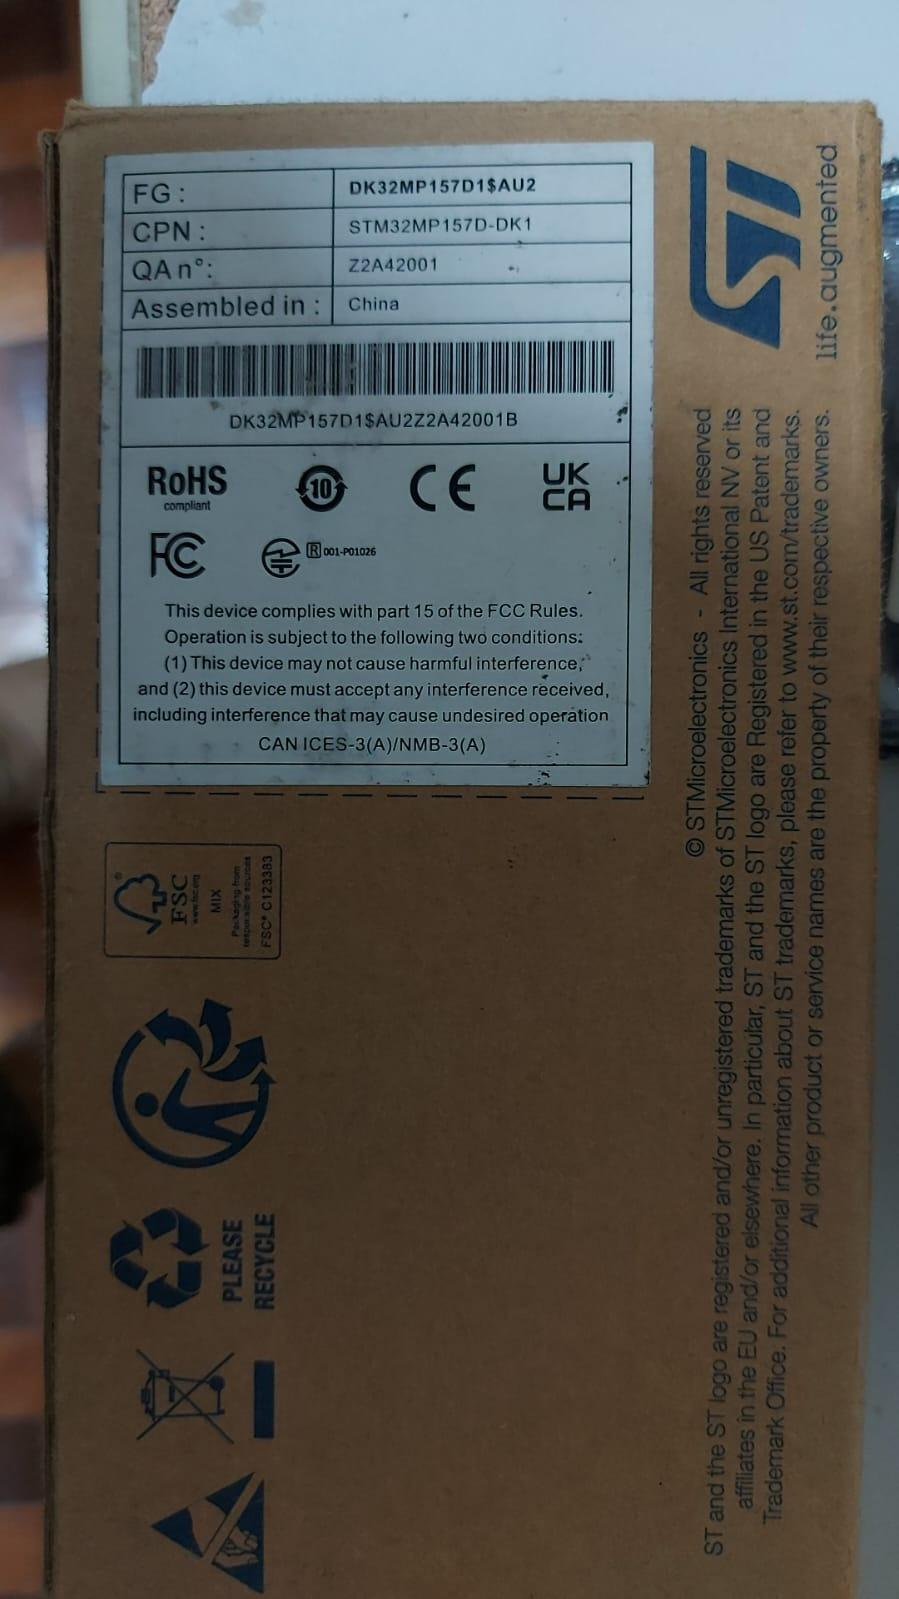
\includegraphics[height=4.6cm]{latex_assets/foto_etiqueta_stm32.jpg}
    \caption{Identificação oficial do kit: Caixa do kit Discovery com etiqueta de conferência (\texttt{KIT STM32MP1 DK1 + CABO USB C + SD CARD}) e etiqueta lateral do fabricante (\texttt{STM32MP157D-DK1}).}
\end{figure}

\subsection{A Placa: STMicroelectronics STM32MP157D-DK1}
Não se trata de um microcontrolador comum (como Arduino ou STM32F1/F4), mas de um \textbf{Microprocessador (MPU) Híbrido}:
\begin{itemize}[leftmargin=*]
    \item \textbf{Dual Arm Cortex-A7 @ 800 MHz:} Processador principal de 32 bits que roda um \textbf{Sistema Operacional Linux Completo} gravado no cartão microSD. É nesse ambiente Linux em espaço de usuário que a sua aplicação C++ vai executar.
    \item \textbf{Arm Cortex-M4 @ 209 MHz:} Coprocessador interno para tarefas de tempo real crítico.
    \item \textbf{Nível Lógico de 3,3 V:} Todos os barramentos de entrada/saída (GPIOs e conversores A/D) operam estritamente em \textbf{3,3 V}.
\end{itemize}

\subsection{O Sensor: Módulo Infravermelho Reflexivo (HW-201 / LM393)}
O Sensor Nº 3 atribuído ao grupo tem a finalidade de detectar aproximação ou abertura de compartimento através da interrupção/reflexão de luz infravermelha:
\begin{theorybox}{Como o Sensor HW-201 Funciona Fisicamente?}
Na extremidade frontal da plaquinha encontram-se dois elementos ópticos de 5 mm:
\begin{enumerate}[leftmargin=*]
    \item \textbf{Emissor IR (transparente):} Emite continuamente feixes de luz infravermelha.
    \item \textbf{Fototransistor Receptor (preto):} Recebe os feixes de luz que batem em um obstáculo próximo (a tampa do compartimento) e refletem de volta.
    \item \textbf{Comparador LM393 e Trimpot Azul:} O circuito integrado LM393 compara o sinal do receptor óptico com a tensão de referência ajustada pelo parafuso azul (trimpot). O circuito opera em lógica \textbf{Active-Low}:
    \begin{itemize}
        \item \textbf{Tampa Fechada (Reflexão Presente):} O pino de saída \texttt{OUT} vai para \textbf{Nível Lógico BAIXO (0 V)} e o LED indicador da placa acende.
        \item \textbf{Tampa Aberta / Violação (Sem Reflexão):} O feixe infravermelho se propaga livremente, o pino \texttt{OUT} vai para \textbf{Nível Lógico ALTO (3,3 V)} e o LED indicador apaga.
    \end{itemize}
\end{enumerate}
\end{theorybox}

\begin{alertbox}{Regras Críticas de Segurança de Bancada}
\begin{enumerate}[leftmargin=*]
    \item \textbf{Proibição Absoluta do Pino 5V:} O sensor HW-201 deve ser alimentado \textbf{exclusivamente em 3,3 V}. Como a saída \texttt{OUT} acompanha a tensão de alimentação, ligar em 5V injetaria 5V no conversor da placa e causaria \textbf{queima permanente} do chip STM32MP1.
    \item \textbf{Preservação do Cartão microSD:} O cartão inserido na placa contém a imagem oficial do Linux configurada para a disciplina. Nunca o remova da placa.
    \item \textbf{Montagem Totalmente Desenergizada:} É obrigatório desconectar todos os cabos (USB-C, Micro-USB e rede) antes de espetar qualquer jumper.
\end{enumerate}
\end{alertbox}

\newpage
% ====================================================================
\section{Passo 0: A Montagem Física e o Repositório Git (Entrega 0)}
% ====================================================================

\subsection{Mapeamento dos Jumpers Pino a Pino}
Para realizar a ligação segura, utilize \textbf{3 cabos jumper Fêmea-Macho}. Posicione a placa virada de costas (lado com adesivo branco \texttt{USER: root SENHA: root} para cima), deixando os conectores pretos fêmea voltados para você e o slot de cartão microSD apontando para a esquerda:

\begin{figure}[H]
    \centering
    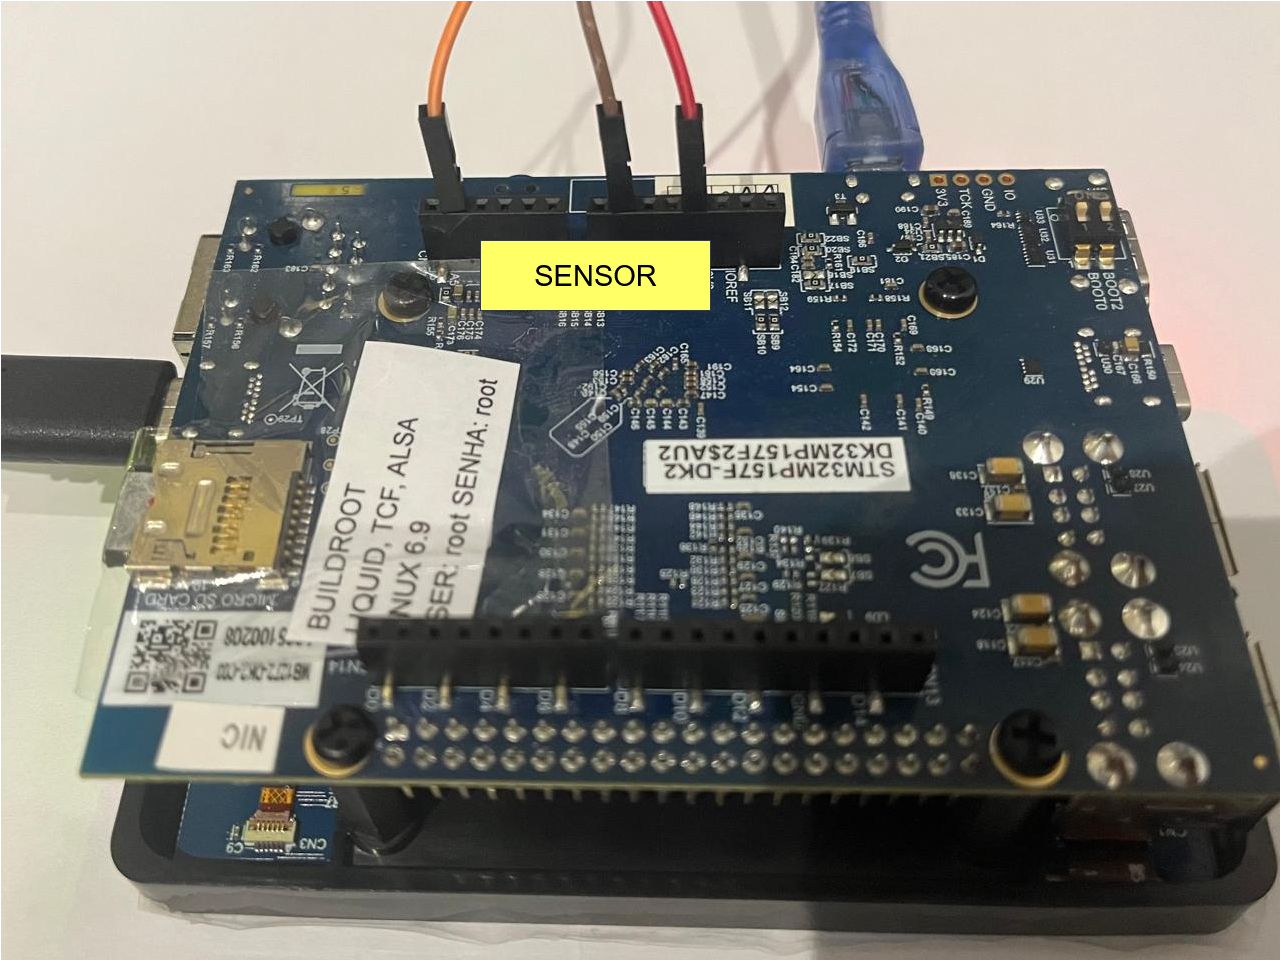
\includegraphics[width=0.48\textwidth]{latex_assets/page9_img1.png}
    \hfill
    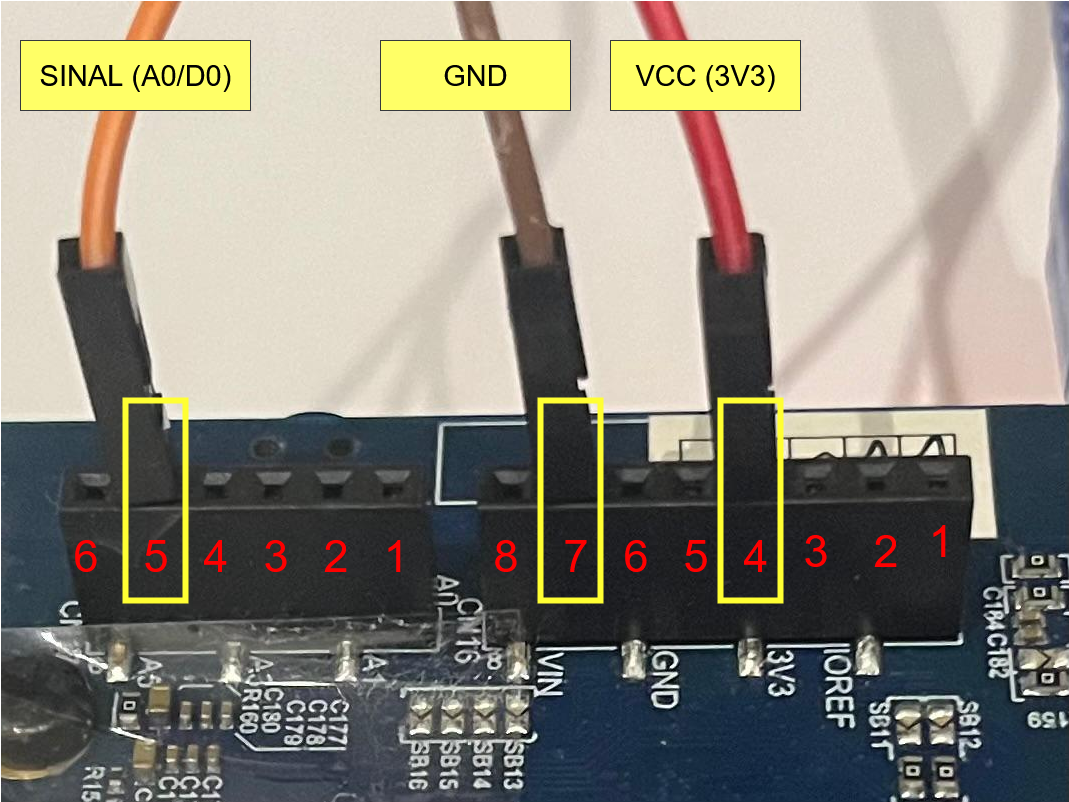
\includegraphics[width=0.48\textwidth]{latex_assets/page9_img2.png}
    \caption{Referência oficial de conexão física (Figuras 4 e 5 do edital): Conexão da alimentação e do sinal analógico contando os furos rigorosamente \textbf{da direita para a esquerda}.}
\end{figure}

\begin{center}
\begin{tabular}{clllp{5.0cm}}
    \toprule
    \textbf{Pino no Sensor} & \textbf{Cor Sugerida} & \textbf{Conector na STM32MP1} & \textbf{Posição Exata} & \textbf{Conferência Visual} \\
    \midrule
    \texttt{VCC} & Vermelho / Cinza & Bloco da Direita (8 furos) & \textbf{Pino 4} (acima de \texttt{3V3}) & Sobram 3 furos vazios à direita dele. \\
    \texttt{GND} & Preto / Branco & Bloco da Direita (8 furos) & \textbf{Pino 7} (acima de \texttt{GND}) & Sobram 2 furos vazios até o fio de 3,3V e 1 furo vazio à esquerda (\texttt{VIN}). \\
    \texttt{OUT} & Laranja / Preto & Bloco da Esquerda (6 furos) & \textbf{Pino 5} (Entrada ADC) & Sobram 4 furos vazios à direita dele e 1 furo vazio na ponta esquerda. \\
    \bottomrule
\end{tabular}
\end{center}

\subsection{Configuração do Repositório Git e Submissão}
A entrega de todas as etapas é realizada via \textbf{link do commit final no GitHub}:
\begin{lstlisting}[language=bash]
# 1. No diretorio do projeto, inicialize o git caso ainda nao o tenha feito
cd c:/Users/jvpar/estudo/3.2/ProgAplicada/projeto_final
git init

# 2. Crie o arquivo .gitignore para evitar comitar arquivos binarios ou pesados
cat << 'EOF' > .gitignore
*.exe
*.o
app_sensor
app_sensor_arm
*.aux
*.log
*.toc
*.out
.vscode/
EOF

# 3. Adicione os arquivos do projeto e faca o primeiro commit
git add include/ src/ Makefile Doxyfile README.md .gitignore docs/
git commit -m "Entrega 1: Classe C++ IrObstacleSensor documentada com Doxygen"

# 4. Vincule ao repositorio oficial no GitHub e envie:
git remote add origin https://github.com/VPariz/stm32-projeto-final-prog-aplicada.git
git branch -M main
git push -u origin main
\end{lstlisting}

\newpage
% ====================================================================
\section{Passo 1: Subsistema IIO, POO e Doxygen (Entrega 1 --- 800 Pontos)}
% ====================================================================

A **Entrega 1** (Figura~\ref{fig:entrega1}) possui prazo em **26/10/2026 às 23:59** e pontuação de **800 pontos**.

\begin{figure}[H]
    \centering
    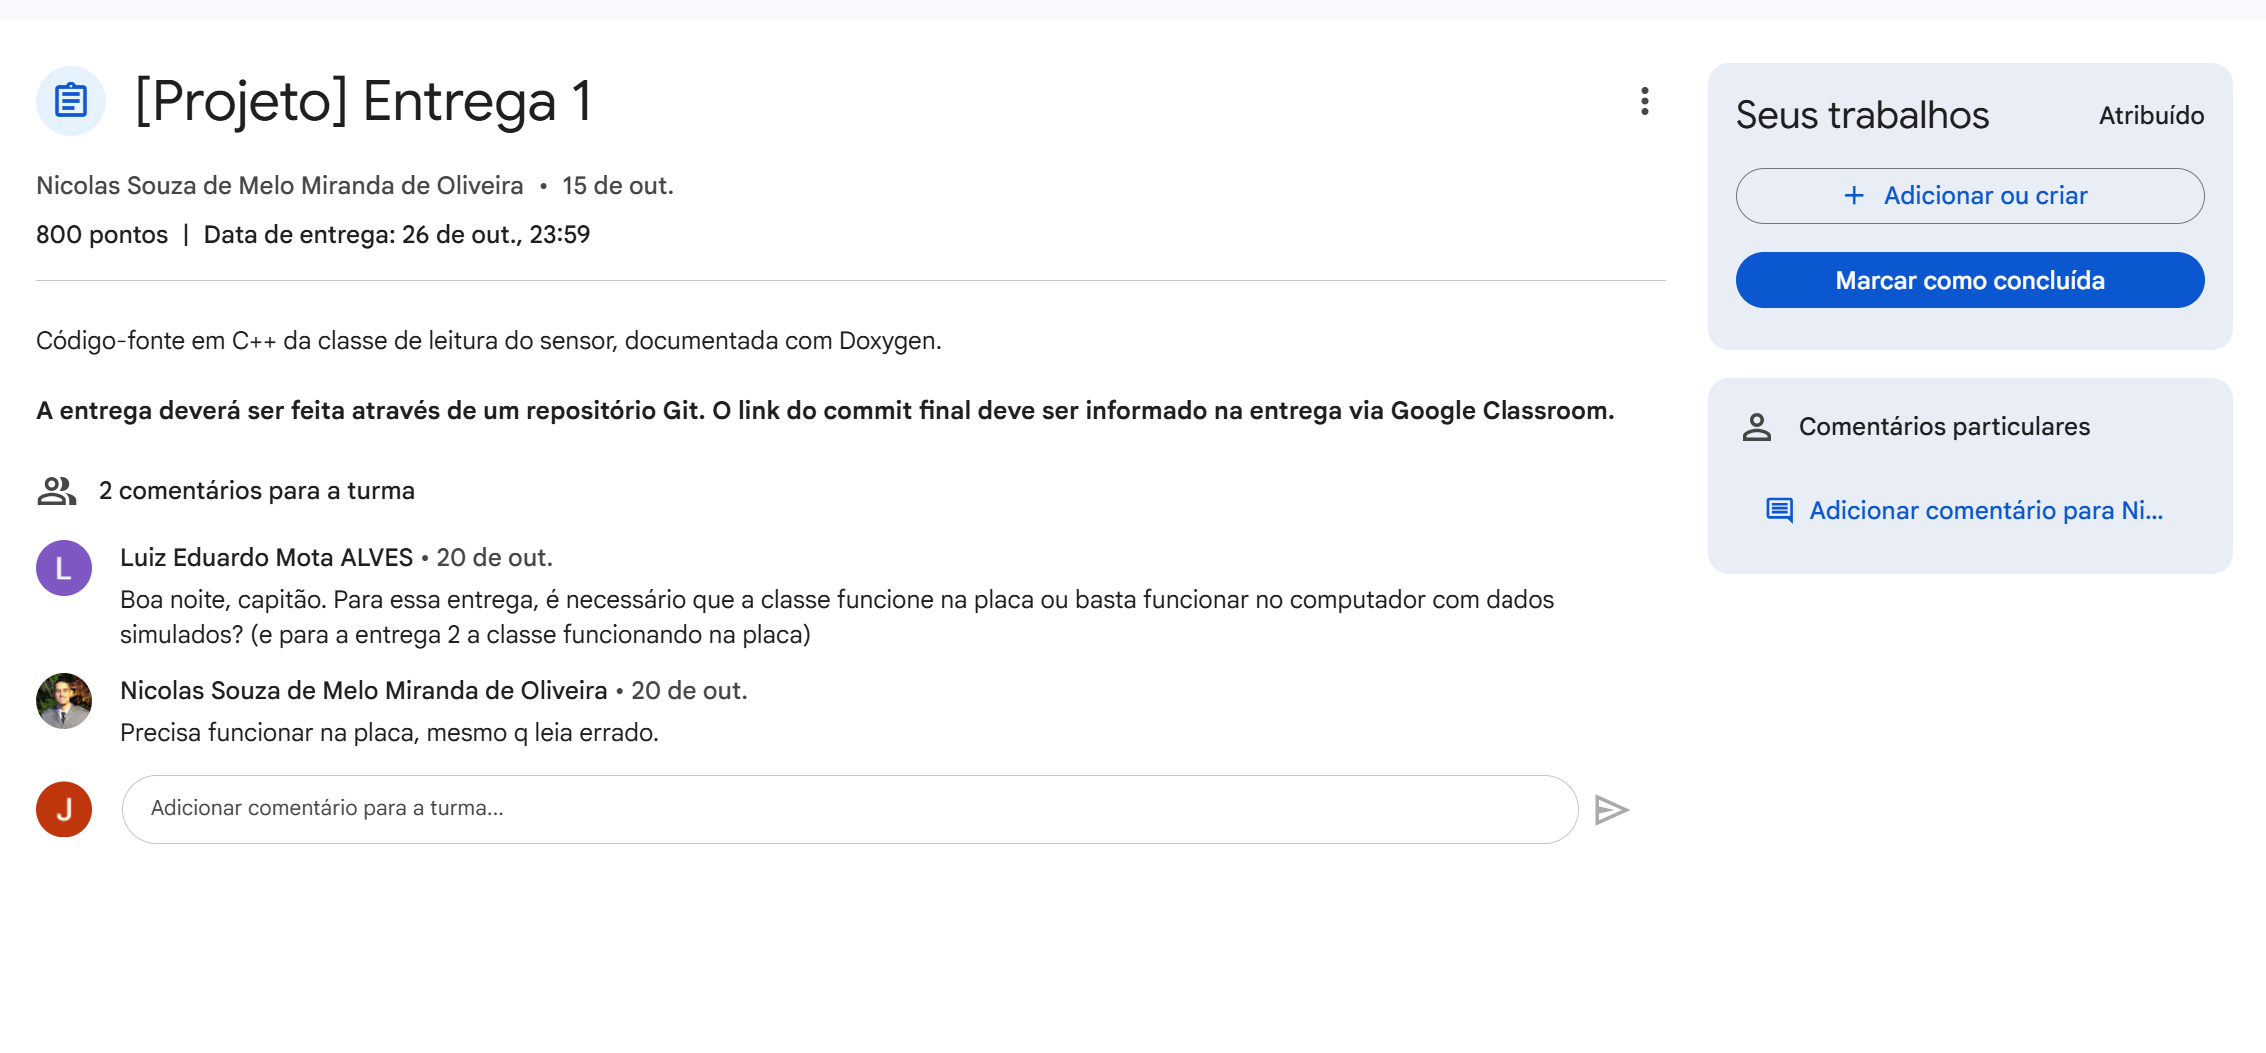
\includegraphics[width=0.88\textwidth]{latex_assets/classroom_entrega1_atualizada.png}
    \caption{Atividade da Entrega 1 no Google Classroom com esclarecimento crítico do corpo docente nos comentários.}
    \label{fig:entrega1}
\end{figure}

\begin{alertbox}{Aviso Crítico do Classroom: Exigência de Execução na Placa}
Na aba de comentários da Entrega 1, um aluno questionou expressamente:
\begin{quote}
    \textit{"Para essa entrega, é necessário que a classe funcione na placa ou basta funcionar no computador com dados simulados?"}
\end{quote}
A resposta oficial do docente foi categórica:
\begin{quote}
    \textbf{"Precisa funcionar na placa, mesmo q leia errado."}
\end{quote}
\textbf{Conclusão de Engenharia:} A classe em C++ não pode ser apenas um protótipo para PC. Ela deve acessar o nó de arquivo virtual do Kernel Linux (\texttt{/sys/bus/iio/...}), ser compilada (ou transferida) para a placa e executar uma leitura real do conversor na STM32MP157D-DK1, mesmo que a calibração final do limiar ocorra na Entrega 2.
\end{alertbox}

\subsection{O Subsistema IIO no Linux (Industrial I/O)}
No Linux da placa STM32MP157D-DK1, o conversor A/D é exposto como arquivo virtual no diretório:
\begin{center}
    \texttt{/sys/bus/iio/devices/iio:device0/}
\end{center}
Dentro dele residem arquivos como \texttt{in\_voltage0\_raw}, \texttt{in\_voltage1\_raw}, etc. Ler esse arquivo equivale a solicitar ao Kernel a leitura analógica imediata no conversor físico.

\subsection{Procedimento Presencial: Descoberta do Canal Exato do ADC}
\begin{figure}[H]
    \centering
    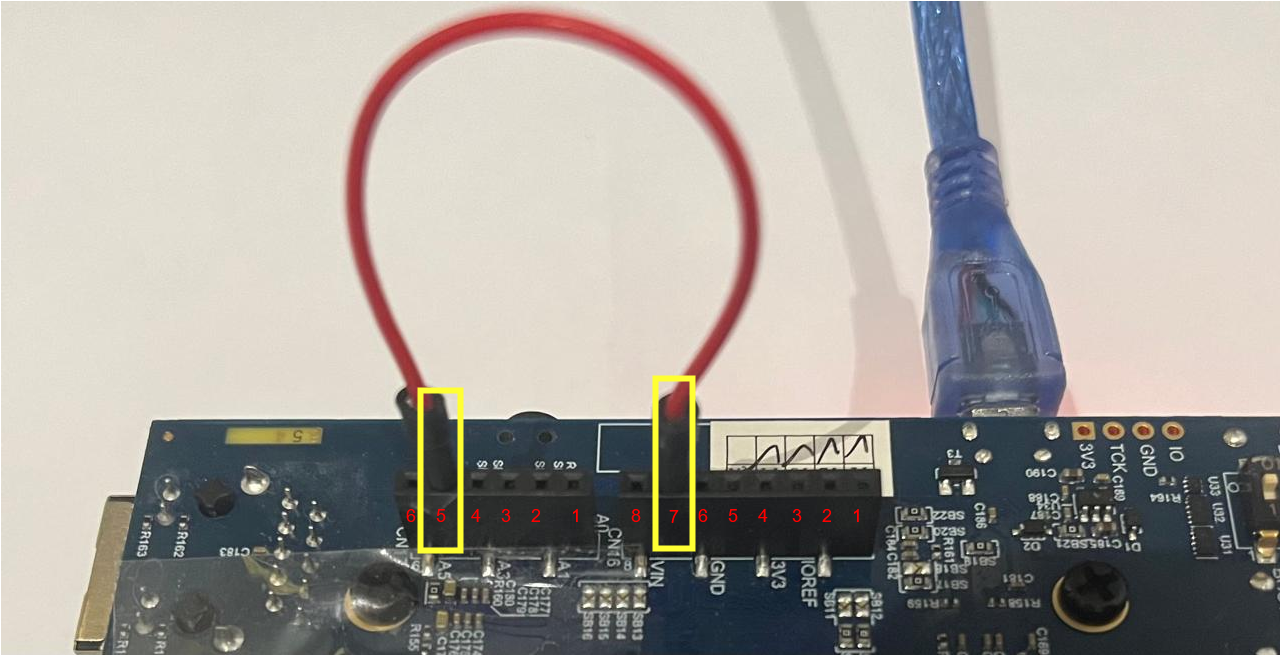
\includegraphics[width=0.62\textwidth]{latex_assets/page8_img1.png}
    \caption{Identificação de canal (Figura 3 do edital): Conexão direta do pino ADC ao GND com jumper para identificação de leitura zero.}
\end{figure}

\begin{labbox}{Roteiro de 5 Minutos no Laboratório}
\begin{enumerate}[leftmargin=*]
    \item Com a placa desligada, coloque um jumper conectando o \textbf{Pino 5 do bloco de 6 furos (ADC)} ao \textbf{Pino 7 (GND)} do bloco de alimentação.
    \item Ligue a placa com o cabo USB-C na porta \texttt{PWR\_IN} e conecte o cabo Micro-USB serial no PC.
    \item Abra o TeraTerm configurado para \textbf{115200 8N1}, aperte Enter e faça login com usuário \texttt{root} e senha \texttt{root}.
    \item No terminal da placa, digite:
\begin{lstlisting}[language=bash]
cd /sys/bus/iio/devices/iio:device0/
cat in_voltage*_raw
\end{lstlisting}
    \item O arquivo \texttt{in\_voltageX\_raw} que retornar \textbf{0} (ou ruído elétrico desprezível, ex.: 1) é o canal do pino testado.
    \item Desligue, reconecte o sensor HW-201 e confira que com a tampa fechada (reflexão) o valor lido é baixo, e com o feixe desimpedido o valor é alto.
\end{enumerate}
\end{labbox}

\subsection{Código da Classe: \texttt{IrObstacleSensor.hpp} e \texttt{IrObstacleSensor.cpp}}
\begin{lstlisting}[language=C++]
// Joao Victor Pariz - Projeto Final - Sensor HW-201 - SE/3 - Eletronica - Programacao Aplicada
#ifndef IR_OBSTACLE_SENSOR_HPP
#define IR_OBSTACLE_SENSOR_HPP

#include <string>
#include <fstream>
#include <stdexcept>
#include <sstream>
#include <iomanip>

/**
 * @file IrObstacleSensor.hpp
 * @brief Classe de leitura e diagnostico do Sensor HW-201 via Industrial I/O (IIO).
 */
class IrObstacleSensor {
private:
    std::string devicePath;      /**< Caminho no sysfs do Linux ou mock para PC */
    int rawThreshold;            /**< Limiar de comutacao entre estado seguro e violado */
    int lastRawValue;            /**< Ultimo valor bruto inteiro lido do ADC */
    double referenceVoltage;     /**< Tensao de referencia eletrica (3.3 V) */
    int maxAdcResolution;        /**< Resolucao maxima da escala do ADC (4095 para 12 bits) */

public:
    explicit IrObstacleSensor(
        const std::string& path = "/sys/bus/iio/devices/iio:device0/in_voltage0_raw",
        int threshold = 2000,
        double vref = 3.3,
        int maxAdc = 4095
    );

    virtual ~IrObstacleSensor() = default;

    int readRaw();                     /**< Efetua a leitura atomica do subsistema IIO */
    double getVoltage() const;         /**< Converte valor inteiro em tensao (V) */
    bool isObstacleDetected() const;   /**< Retorna true se houver reflexao (Active-Low) */
    bool isCompartmentViolated() const;/**< Retorna true se a carga foi aberta */
    std::string getFormattedStatus() const;
    int getLastRawValue() const;
    void setThreshold(int newThreshold);
};

#endif // IR_OBSTACLE_SENSOR_HPP
\end{lstlisting}

\subsection{Documentação Doxygen e Checklist da Entrega 1}
\begin{enumerate}[leftmargin=*]
    \item Execute \texttt{doxygen Doxyfile} na pasta raiz do projeto. A documentação será compilada na pasta \texttt{docs/doxygen/html/}.
    \item Abra o arquivo \texttt{docs/doxygen/html/index.html} no navegador e comprove que a classe \texttt{IrObstacleSensor} e todos os seus métodos públicos e privados estão documentados.
    \item Teste a compilação cruzada ou nativa da aplicação:
\begin{lstlisting}[language=bash]
# Compilacao nativa no PC com simulador
g++ -Wall -Wextra -std=c++17 -Iinclude src/IrObstacleSensor.cpp src/main.cpp -o app_sensor
./app_sensor mock_sensor.txt 127.0.0.1 5000 5
\end{lstlisting}
    \item Realize o commit no Git com a tag ou mensagem da Entrega 1 e submeta o link do commit no Google Classroom.
\end{enumerate}

\newpage
% ====================================================================
\section{Passo 2: Compilação Cruzada, Deploy e Execução (Entrega 2 --- 800 Pontos)}
% ====================================================================

A **Entrega 2** (Figura~\ref{fig:entrega2}) possui prazo em **02/11/2026 às 23:59** e pontuação de **800 pontos**.

\begin{figure}[H]
    \centering
    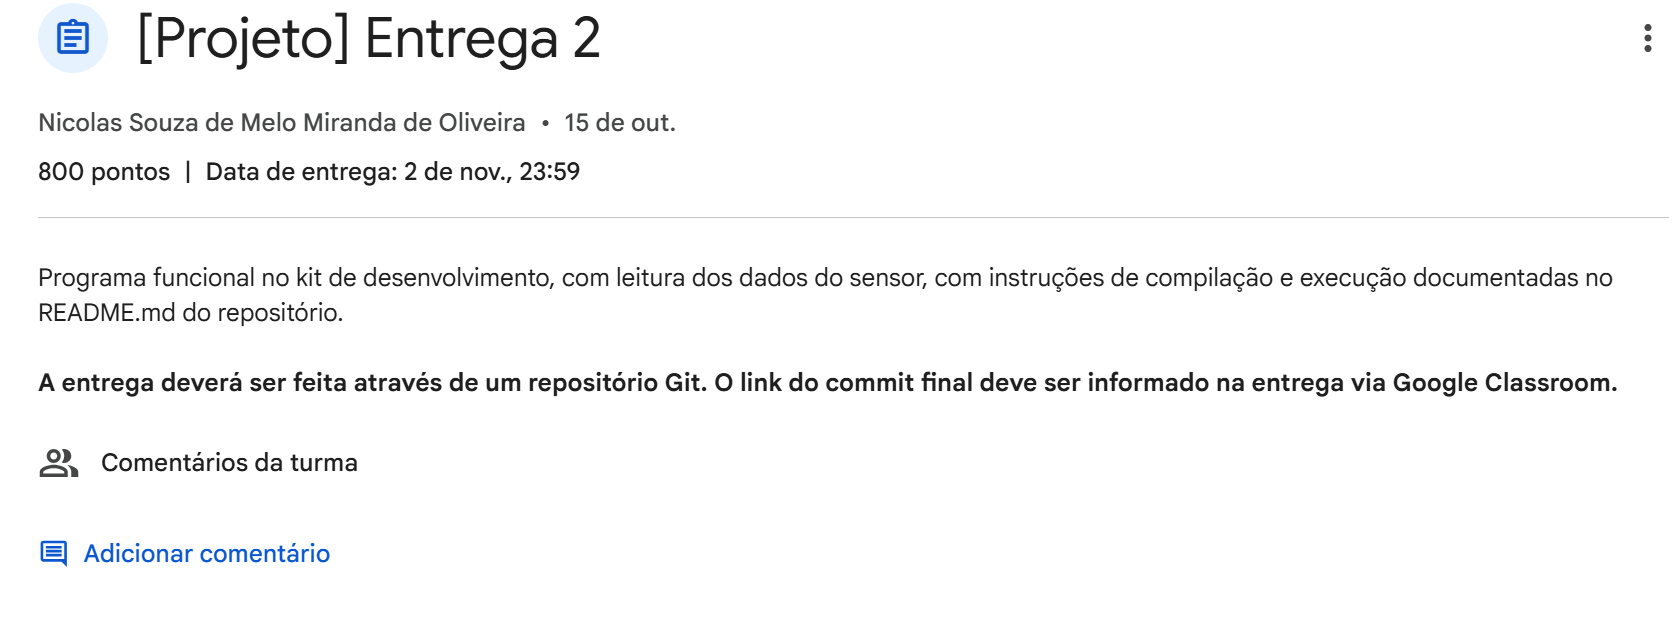
\includegraphics[width=0.88\textwidth]{latex_assets/classroom_entrega2_atualizada.png}
    \caption{Atividade da Entrega 2 no Google Classroom: Programa funcional no kit STM32MP157D-DK1 com documentação no README.md.}
    \label{fig:entrega2}
\end{figure}

\subsection{Fundamentos da Cross-Compilação e Deploy com WinSCP}
Como o computador possui processador x86\_64 e a placa possui um processador Arm Cortex-A7 de 32 bits, usamos a toolchain para gerar o binário \texttt{app\_sensor\_arm}:
\begin{lstlisting}[language=bash]
# Na VM Linux com a toolchain instalada:
make cross
# O executavel 'app_sensor_arm' sera gerado na pasta
\end{lstlisting}

\subsection{Transferência para a Placa e Calibração do Trimpot}
\begin{enumerate}[leftmargin=*]
    \item No WinSCP, conecte no IP \texttt{192.168.42.2} (usuário \texttt{root}, senha \texttt{root}) e arraste \texttt{app\_sensor\_arm} para \texttt{/home/root/}.
    \item No terminal da placa via SSH (\texttt{ssh root@192.168.42.2}) ou serial:
\begin{lstlisting}[language=bash]
chmod +x app_sensor_arm
./app_sensor_arm
\end{lstlisting}
    \item Ajuste a sensibilidade do sensor girando o trimpot azul com uma chave de fenda até que a reflexão com a tampa a 2~cm comute o valor de leitura.
    \item Tire prints do terminal comprovando a alternância entre \texttt{[STATUS: SEGURO]} e \texttt{[STATUS: VIOLADO]} e documente no \texttt{README.md}.
\end{enumerate}

\newpage
% ====================================================================
\section{Passo 3: Telemetria via Socket UDP (Entrega 3 --- 800 Pontos)}
% ====================================================================

A **Entrega 3** (Figura~\ref{fig:entrega3}) possui prazo em **09/11/2026 às 23:59** e pontuação de **800 pontos**.

\begin{figure}[H]
    \centering
    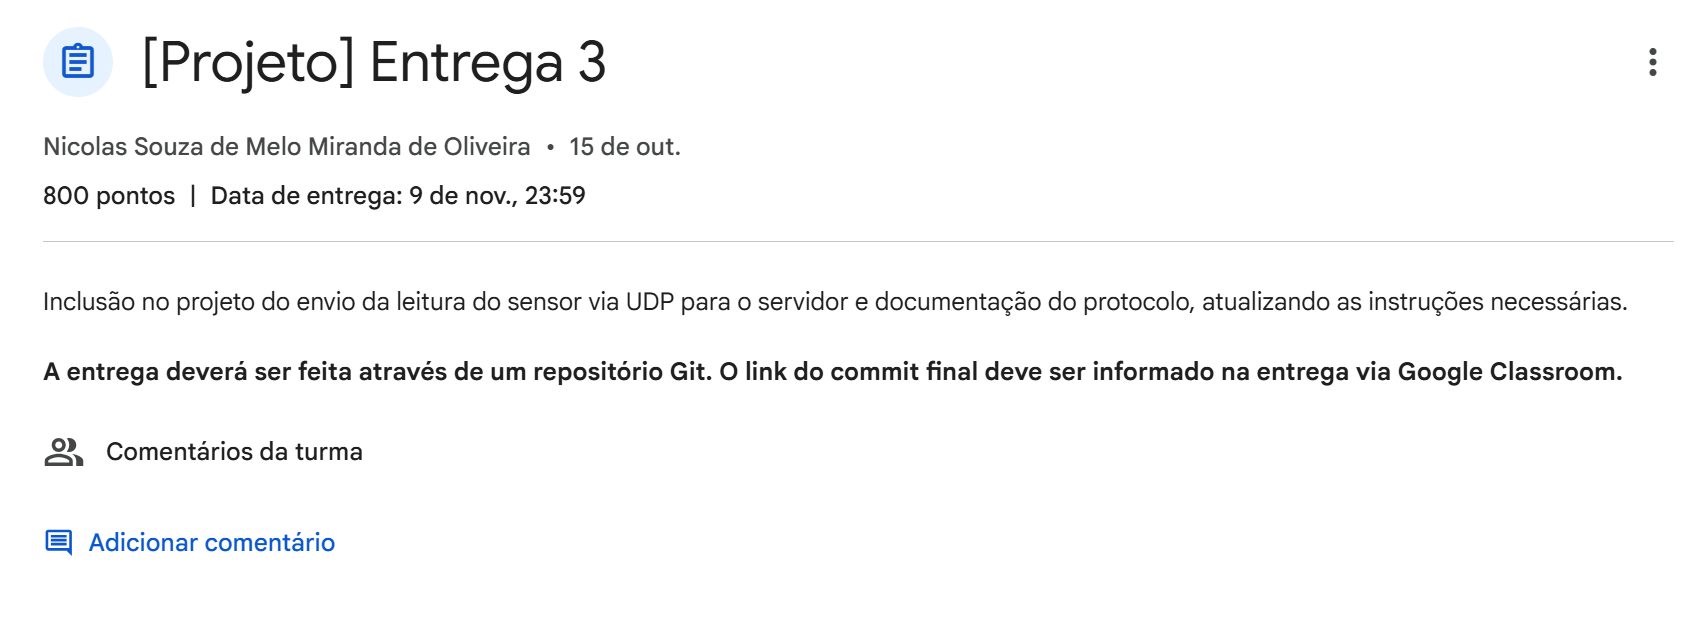
\includegraphics[width=0.88\textwidth]{latex_assets/classroom_entrega3_atualizada.png}
    \caption{Atividade da Entrega 3: Transmissão da leitura do sensor via pacotes UDP para o servidor com protocolo documentado.}
    \label{fig:entrega3}
\end{figure}

\subsection{A Classe \texttt{UdpTransmitter} e o Protocolo de Rede}
A classe \texttt{UdpTransmitter} encapsula sockets POSIX/WinSock, transmitindo datagramas UDP para a porta 5000 do computador central. O formato JSON transmitido é:
\begin{lstlisting}
{
  "sensor_id": "G3_IR_HW201",
  "raw_value": 3840,
  "voltage_v": 3.09,
  "is_violated": true,
  "status_text": "VIOLADO",
  "timestamp_ms": 1729801234567
}
\end{lstlisting}

\newpage
% ====================================================================
\section{Passos 4 e 5: Interface Gráfica, Vídeo e Apresentação (800 + 800 Pontos)}
% ====================================================================

As **Entregas 4 e 5** (Figuras~\ref{fig:entrega4} e~\ref{fig:entrega5}) compartilham a data final de entrega: **16/11/2026 às 23:59**.

\begin{figure}[H]
    \centering
    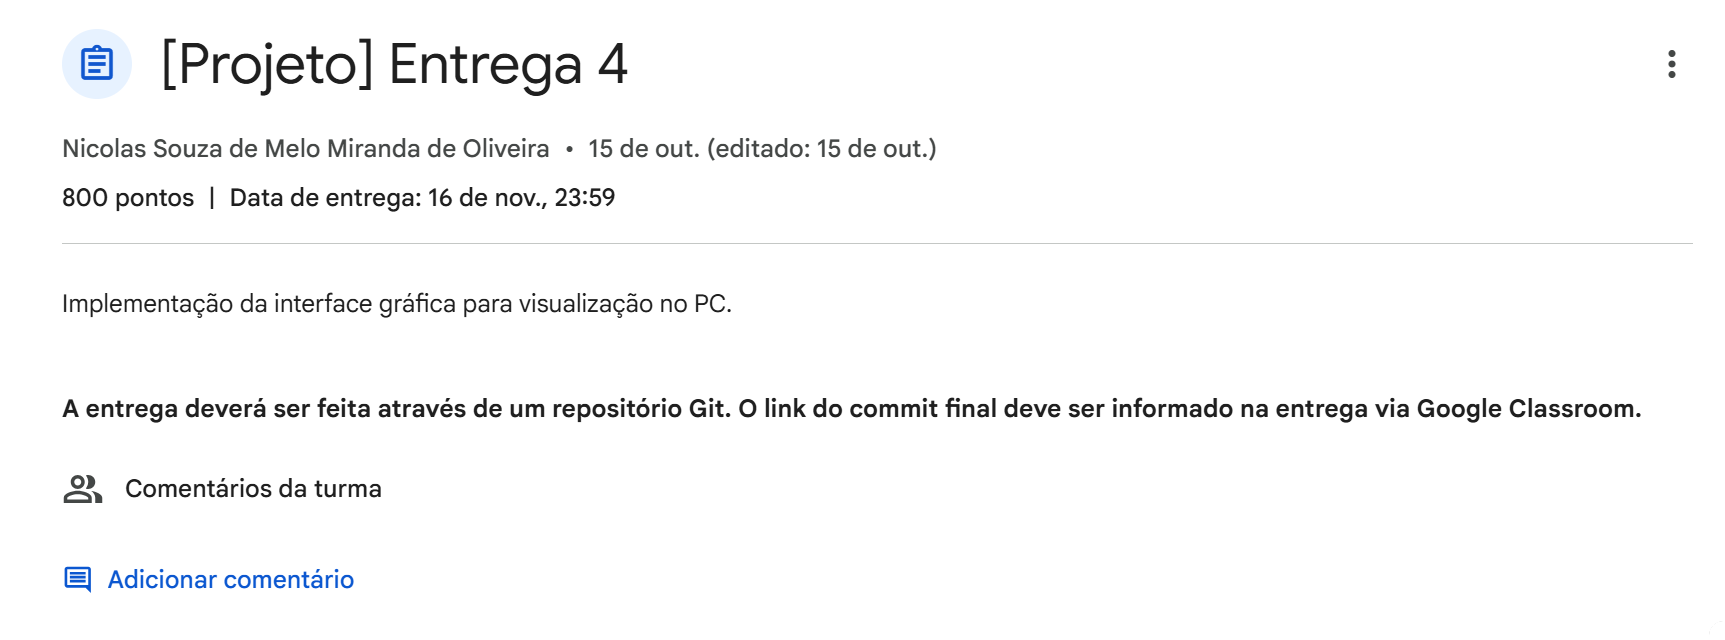
\includegraphics[width=0.88\textwidth]{latex_assets/classroom_entrega4_atualizada.png}
    \caption{Atividade da Entrega 4: Interface gráfica de supervisão no PC.}
    \label{fig:entrega4}
\end{figure}

\begin{figure}[H]
    \centering
    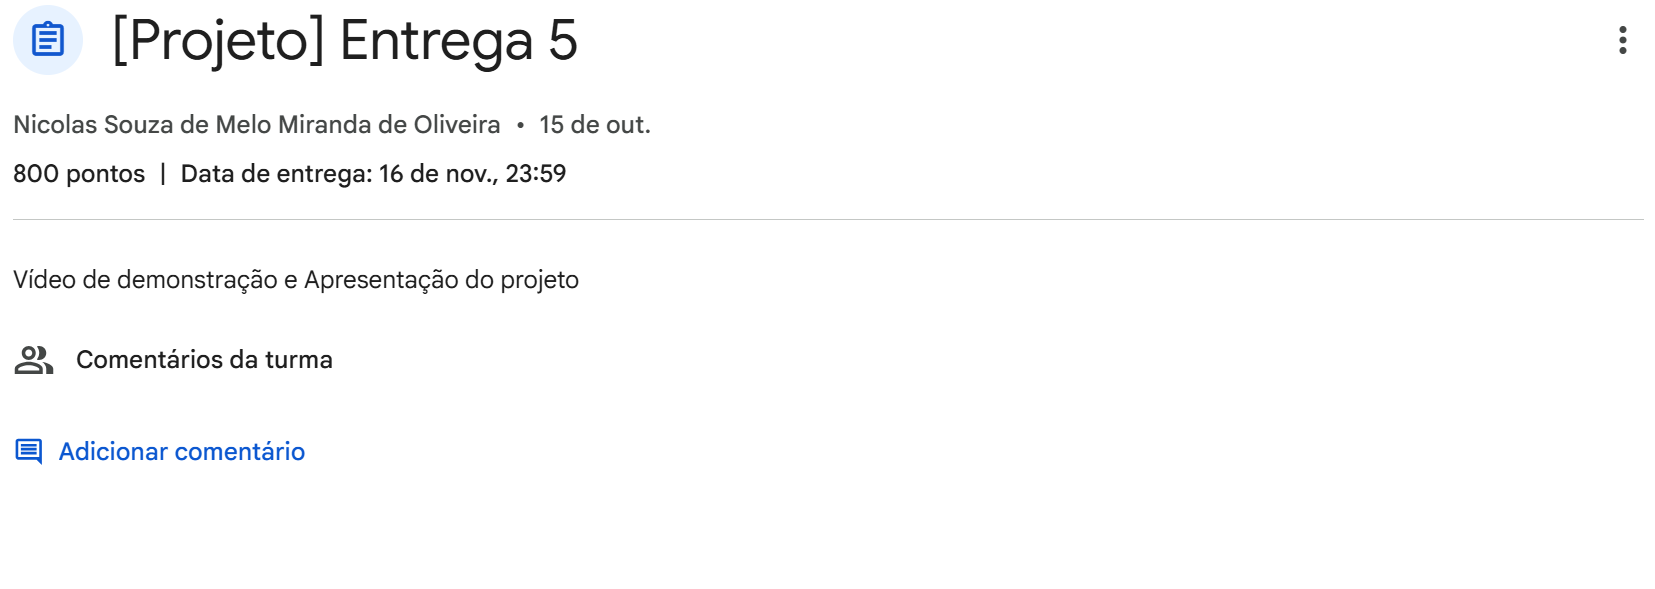
\includegraphics[width=0.88\textwidth]{latex_assets/classroom_entrega5_atualizada.png}
    \caption{Atividade da Entrega 5: Apresentação e vídeo de demonstração do sistema integrado.}
    \label{fig:entrega5}
\end{figure}

\subsection{Dashboard Gráfico em Python (\texttt{scripts/gui\_dashboard.py})}
O script de interface gráfica escuta na porta UDP 5000 e plota um gráfico deslizante dos últimos 60 segundos com Matplotlib/Tkinter, gerando alarme sonoro/visual em caso de violação e salvando o log contínuo em CSV.

\newpage
% ====================================================================
\section{Matriz Consolidada de Entregáveis: O que está Pronto vs. O que Falta Fazer}
% ====================================================================

A tabela a seguir apresenta o status minucioso de cada componente do Projeto Final:

\begin{center}
\begin{tabular}{lp{9.5cm}c}
    \toprule
    \textbf{Etapa} & \textbf{Itens Exigidos e Ações Necessárias} & \textbf{Status Atual} \\
    \midrule
    \textbf{Entrega 0} & Conexão física com placa desligada; fotos dos jumpers de 3,3V, GND e ADC; repositório GitHub criado com integrantes. & \textbf{CONCLUÍDO} \\
    \midrule
    \textbf{Entrega 1} & $\checkmark$ Código em C++ da classe \texttt{IrObstacleSensor} com POO estrita. \newline
    $\checkmark$ Documentação Doxygen completa em \texttt{docs/doxygen/html/}. \newline
    $\square$ Executar \texttt{git init} em \texttt{projeto\_final/}, comitar e enviar para o GitHub. \newline
    $\square$ Submeter a URL do commit final no Google Classroom (Prazo: 26/10). \newline
    $\square$ Garantir teste presencial na placa lendo o nó do IIO. & \textbf{PRONTO P/ ENVIO} \\
    \midrule
    \textbf{Entrega 2} & $\checkmark$ Código funcional pronto para compilação ARM. \newline
    $\square$ Compilação cruzada (\texttt{make cross}) gerando \texttt{app\_sensor\_arm}. \newline
    $\square$ Transferir via WinSCP para a placa e calibrar trimpot do HW-201. \newline
    $\square$ Prints da execução no terminal documentados no \texttt{README.md}. & \textbf{CÓDIGO PRONTO} \\
    \midrule
    \textbf{Entrega 3} & $\checkmark$ Classe \texttt{UdpTransmitter} implementada em C++. \newline
    $\checkmark$ Scripts de teste de recepção UDP em Python implementados. \newline
    $\square$ Teste do fluxo UDP completo placa $\rightarrow$ PC e commit final. & \textbf{CÓDIGO PRONTO} \\
    \midrule
    \textbf{Entrega 4} & $\checkmark$ Interface gráfica em Python (\texttt{gui\_dashboard.py}) pronta com gráfico temporal e exportação CSV. \newline
    $\square$ Capturas da tela do dashboard operando com dados reais. & \textbf{CÓDIGO PRONTO} \\
    \midrule
    \textbf{Entrega 5} & $\square$ Gravação do vídeo de demonstração (3 a 5 min) mostrando o sensor sendo acionado e o alerta no PC. \newline
    $\square$ Apresentação final do projeto. & \textbf{ROTEIRO PRONTO} \\
    \bottomrule
\end{tabular}
\end{center}

\vspace{0.4cm}
\begin{center}
    \rule{0.6\textwidth}{0.4pt}\\[0.2cm]
    {\small \textbf{SE/3 --- Eletrônica --- Programação Aplicada à Engenharia Elétrica --- IME 2026}}
\end{center}

\end{document}
